\documentclass{article}
\usepackage{float}
\usepackage{graphicx}
\usepackage[export]{adjustbox}
\usepackage[english]{babel}
\usepackage{booktabs}
\usepackage{float}
% Set page size and margins
% Replace `letterpaper' with `a4paper' for UK/EU standard size
\usepackage[letterpaper,top=2cm,bottom=2cm,left=3cm,right=3cm,marginparwidth=1.75cm]{geometry}

% Useful packages
\usepackage{amsmath}
\usepackage{graphicx}
\usepackage[colorlinks=true, allcolors=blue]{hyperref}

\title{ZNEUS Project 2}
\author{Amal Akhmadinurov, Lukáš Šebök}

\begin{document}
\maketitle

\section{Tools}

\begin{itemize}
	\item Torch
	\item TorchMetrics
	\item Pandas
	\item Other utility libraries
	
\end{itemize}

\section{Dataset: TIGER Challenge dataset}
\begin{figure}[H]
    \noindent\makebox[\textwidth][c]{%
        \includegraphics[width=0.85\textwidth]{images/tiger-original-ratio-pixels.png}%
    }
    \caption{ Class ratio }
    \label{fig:figure2}
\end{figure}
For this project we used ROI subfolder of this dataset

In each ROI, the following regions are annotated, with the corresponding labels:

\begin{itemize}
    \item \textbf{Invasive tumor} (\textit{label} = 1): this class contains regions of the invasive tumor, including several morphological subtypes, such as invasive ductal carcinoma and invasive lobular carcinoma.
    
    \item \textbf{Tumor-associated stroma} (\textit{label} = 2): this class contains regions of stroma (i.e., connective tissue) that are associated with the tumor. This includes stromal regions within the main bulk of the tumor and its close surroundings. In some cases, the tumor-associated stroma may resemble the “healthy” stroma typically found outside the tumor bulk.
    
    \item \textbf{In-situ tumor} (\textit{label} = 3): this class contains regions of in-situ malignant lesions, such as ductal carcinoma in situ (DCIS) or lobular carcinoma in situ (LCIS).
    
    \item \textbf{Healthy glands} (\textit{label} = 4): this class contains regions of glands with healthy epithelial cells.
    
    \item \textbf{Necrosis not in-situ} (\textit{label} = 5): this class contains regions of necrotic tissue that are not part of in-situ tumor. For example, DCIS often presents a typical necrotic pattern that is considered part of the lesion itself; such necrotic regions are annotated as “in-situ tumor” rather than “necrosis.”
    
    \item \textbf{Inflamed stroma} (\textit{label} = 6): this class contains tumor-associated stroma with a high density of lymphocytes (i.e., “inflamed”). For TIL assessment, inflamed stroma and tumor-associated stroma may be grouped together, but they were annotated separately to account for differences in visual patterns.
    
    \item \textbf{Rest} (\textit{label} = 7): this class contains various tissue compartments not specifically annotated in the other categories; examples include healthy stroma, erythrocytes, adipose tissue, skin, nipple, etc.
\end{itemize}





\begin{figure}[H]
    \noindent\makebox[\textwidth][c]{%
        \includegraphics[width=0.65\textwidth]{images/tiger-example.png}%
    }
    \caption{ Visualization of TIGER dataset }
    \label{fig:figure2}
\end{figure}


\subsection{Normalization and data transformation}

Each image was normilized using division by 255.

\subsubsection*{Patches}
To make dataset larger and leverage large images in the dataset we have decided to extract 256x256 non-overlapping patches from original images. Images that have size smaller than patch size were non patched, but only resized to 256x256.

\subsubsection*{Augmentations}
For each image we have applied the following tranformations:
\begin{itemize}
    \item \textbf{Rotate}: Random rotation with a limit of $45^\circ$, using the specified \texttt{border\_mode} ($p = 0.5$).
    \item \textbf{ShiftScaleRotate}: Applies random shifting (up to $0.5$), scaling (up to $0.15$), and no rotation, with the given \texttt{border\_mode} ($p = 0.5$).
    \item \textbf{HorizontalFlip}: Random horizontal flip applied with probability $0.5$.
    \item \textbf{VerticalFlip}: Random vertical flip applied with probability $0.5$.
\end{itemize}

\subsubsection*{BORDER REFLECT}

During EDA we have identified that augmentations create a big amount of pixels with 0 value. To address this issue that will inevitably harm the performance of the model we have used border reflect mode (from OpenCV library). Examples of augmented images can be seen in figure 3 

\begin{figure}[H]
    \noindent\makebox[\textwidth][c]{%
        \includegraphics[width=0.8\textwidth]{images/aug-example.png}%
    }
    \caption{ Model architecture without pretrained backbone}
    \label{fig:figure2}
\end{figure}

\section{Evaluation Metrics}

The model evaluates performance using the following metrics, computed for both training and validation sets:

\begin{itemize}
    \item \textbf{IoU}: Mean Intersection over Union across all classes, computed using \texttt{MeanIoU} with \texttt{include\_background=True} and \texttt{input\_format="index"}.
    \item \textbf{Dice Score}: Macro-averaged Dice coefficient, computed using \texttt{DiceScore} with \texttt{include\_background=True}, \texttt{average="macro"}, and \texttt{input\_format="index"}.
    \item \textbf{Loss}: Segmentation loss defined by the chosen loss function $\mathcal{L}$, applied to logits and class-index masks.
\end{itemize}
\section{Original Tiger Dataset experiments}
Report  is available here: \href{https://wandb.ai/amal-akhmadinurov-stu/zneus-tiger-u-net/reports/Tiger-Dataset-Segmentation-Report--VmlldzoxNTI2NzIzNA?accessToken=3al9pnc4jqedkva9eu8tdnspt23t4mr5io13gt3dfxya8c7c5mca3j2ddm89c59n}{Report}
\subsection{Model Architecture}

Initially we have used model without any pretrained backbone.
\begin{figure}[H]
    \noindent\makebox[\textwidth][c]{%
        \includegraphics[width=0.85\textwidth]{images/out-u-net.png}%
    }
    \caption{ Model architecture without pretrained backbone}
    \label{fig:figure2}
\end{figure}

But for further experiments we used layers from a pretrained version of EfficiientNetB0

\begin{figure}[H]
    \noindent\makebox[\textwidth][c]{%
        \includegraphics[width=0.85\textwidth]{images/efficiient-backbone-u-net.drawio.png}%
    }
    \caption{ Model architecture with EfficientNetB0 based pretrained encoder (best model in experiments)}
    \label{fig:figure2}
\end{figure}



\subsection{Hyperparameters}

The best model uses EfficientNetB0 pretrained layers for the encoder part and custom decoder trained from the ground up (look at Figure 2 for architecture) with  the following hyperparameters, defined as constants in the implementation:

\begin{table}[h]
\centering
\caption{Hyperparameters of the Model}
\begin{tabular}{l c}
\toprule
\textbf{Parameter} & \textbf{Value} \\
\midrule
Batch Size & 32 \\
Learning Rate & 0.001 \\
Maximum Epochs & 50 \\
Reduce LR Patience & 10 \\
Early Stopping Patience & 10 \\
Loss function & JaccardLoss("multiclass", [1,2,3,4,5,6,7]) \\
Image Size & 256x256 \\
\bottomrule
\end{tabular}
\end{table}

Loss function is Jaccard Loss (class is imported from segmentation\_models\_pytorch library) includes only 7 classes in the computation as 0 class is undefined in the original dataset.

The model applies a argmax activation to the output logits during training and evaluation to produce probabilities for each class in the output mask.

 Key takeaways from this group of experiments:
\begin{itemize}
	\item Image size can seriously influence the performance
	\item Original Dataset is imbalanced
	\item In out case its makes sense to use pretrained backbone

	
\end{itemize}
 

\subsection{Results}

\begin{table}[H]
\centering
\begin{tabular}{l c}
\hline
\textbf{Class} & \textbf{Count} \\
\hline
Loss: & 0.48958 \\
IOU & 0.43021 \\
Dice Score & 0.5933 \\

\hline
\end{tabular}
\caption{Best metrics values achieved on validation set}
\end{table}



\begin{figure}[H]
    \noindent\makebox[\textwidth][c]{%
        \includegraphics[width=1.0\textwidth]{images/efficient-net-tiger.png}%
    }
    \caption{ Confusion matrix in percents (per pixels)}
    \label{fig:figure2}
\end{figure}


\begin{figure}[H]
    \noindent\makebox[\textwidth][c]{%
        \includegraphics[width=0.80\textwidth]{images/output-eff-tiger.png}%
    }
    \caption{ Example output on validation set}
    \label{fig:figure2}
\end{figure}

\pagebreak

\section{Modified Dataset: Unicorn Challenge Task 9. U-Net with EfficientNet encoder }
Report  is available here: \href{https://wandb.ai/amal-akhmadinurov-stu/zneus-tiger-u-net-3-classes/reports/Unicorn-Task-9-dataset---VmlldzoxNTI2OTA4MQ?accessToken=g106vrq96cbmkjg52gccwxgr8o2ygth8w1vyq3xb8q82vs6ipxca3lmpxhqtzxao}{Report}

\subsection{Data tranformation}

The original seven annotated tissue classes from TIGER were merged into three:

\begin{itemize}
    \item Invasive tumor and in-situ tumor $\rightarrow$ \textbf{tumor}
    \item Tumor-associated stroma and inflamed stroma $\rightarrow$ \textbf{stroma}
    \item Healthy glands, necrosis not in-situ, and rest $\rightarrow$ \textbf{rest}
\end{itemize}


\begin{figure}[H]
    \noindent\makebox[\textwidth][c]{%
        \includegraphics[width=0.75\textwidth]{images/unicorn-ratio.png}%
    }
    \caption{ Best model architecture with EfficientNetB0 based pretrained encoder}
    \label{fig:figure2}
\end{figure}

\subsection{Model Architecture}


For these experiments we used layers from a pretrained version of EfficiientNetB0 for encoder of the U-Net and custom decoder.

\begin{figure}[H]
    \noindent\makebox[\textwidth][c]{%
        \includegraphics[width=0.85\textwidth]{images/efficiient-backbone-u-net-task9.drawio.png}%
    }
    \caption{ Best model architecture with EfficientNetB0 based pretrained encoder}
    \label{fig:figure2}
\end{figure}



\subsection{Hyperparameters}

The best model uses EfficientNetB0 pretrained layers for the encoder part and custom decoder trained from the ground up (look at Figure 8 for architecture) with  the following hyperparameters, defined as constants in the implementation:

\begin{table}[h]
\centering
\caption{Hyperparameters of the Model}
\begin{tabular}{l c}
\toprule
\textbf{Parameter} & \textbf{Value} \\
\midrule
Batch Size & 32 \\
Learning Rate & 0.001 \\
Maximum Epochs & 50 \\
Reduce LR Patience & 10 \\
Early Stopping Patience & 10 \\
Loss function & JaccardLoss("multiclass", [0,1,2]) \\
Image Size & 256x256 \\
\bottomrule
\end{tabular}
\end{table}

Loss function is Jaccard Loss (class is imported from segmentation\_models\_pytorch library) 
The model applies a argmax activation to the output logits during training and evaluation to produce probabilities for each class in the output mask.

 Key takeaways from this group of experiments:
\begin{itemize}
	\item Image size can seriously influence the performance
	\item Original Dataset is imbalanced
	\item In out case its makes sense to use pretrained backbone

	
\end{itemize}
 

\subsection{Results}

\begin{table}[H]
\centering
\begin{tabular}{l c}
\hline
\textbf{Class} & \textbf{Count} \\
\hline
Loss: & 0.24133 \\
IOU & 0.57794 \\
Dice Score & 0.713 \\

\hline
\end{tabular}
\caption{Best metrics values achieved on validation set}
\end{table}



\begin{figure}[H]
    \noindent\makebox[\textwidth][c]{%
        \includegraphics[width=1.0\textwidth]{images/conf-task-9.png}%
    }
    \caption{ Confusion matrix in percents (per pixels)}
    \label{fig:figure2}
\end{figure}

\begin{figure}[H]
    \noindent\makebox[\textwidth][c]{%
        \includegraphics[width=0.80\textwidth]{images/eff-conf-non-h.png}%
    }
    \caption{ Confusion matrix in percents (per pixels) for only non-homogenious patches}
    \label{fig:figure2}
\end{figure}

\begin{figure}[H]
    \noindent\makebox[\textwidth][c]{%
        \includegraphics[width=0.80\textwidth]{images/output-eff-task-9.png}%
    }
    \caption{ Example output on validation set}
    \label{fig:figure2}
\end{figure}


\begin{figure}[H]
    \noindent\makebox[\textwidth][c]{%
        \includegraphics[width=1.0\textwidth]{images/conf-task-9.png}%
    }
    \caption{ Confusion matrix in percents (per pixels)}
    \label{fig:figure2}
\end{figure}






\pagebreak

\section{Modified Dataset: Unicorn Challenge Task 9. Attention U-Net }
Report  is available here: \href{https://wandb.ai/amal-akhmadinurov-stu/zneus-tiger-u-net/reports/Tiger-Dataset-Segmentation-Report--VmlldzoxNTI2NzIzNA?accessToken=3al9pnc4jqedkva9eu8tdnspt23t4mr5io13gt3dfxya8c7c5mca3j2ddm89c59n}{Report} (contains also future  experiments)

As a part of this experiments we also tested training only on non-homogenious patches (patches that contains several classes) because there is a big amount of patches that contain only one class, that makes our model to do classification task rather than real segmentation.
\subsection{Model Architecture}


For these experiments we used layers from a pretrained version of EfficiientNetB0 for encoder of the U-Net and custom decoder with applied attention mechanism.

\begin{figure}[H]
    \noindent\makebox[\textwidth][c]{%
        \includegraphics[width=1.0\textwidth]{images/u-net-attention.drawio.png}%
    }
    \caption{ Confusion matrix in percents (per pixels)}
    \label{fig:figure2}
\end{figure}



\subsection{Hyperparameters}

The best model uses EfficientNetB0 pretrained layers for the encoder part and custom decoder trained from the ground up (look at Figure 8 for architecture) with  the following hyperparameters, defined as constants in the implementation:

\begin{table}[h]
\centering
\caption{Hyperparameters of the Model}
\begin{tabular}{l c}
\toprule
\textbf{Parameter} & \textbf{Value} \\
\midrule
Batch Size & 32 \\
Learning Rate & 0.001 \\
Maximum Epochs & 50 \\
Reduce LR Patience & 10 \\
Early Stopping Patience & 10 \\
Loss function & JaccardLoss("multiclass", [0,1,2]) \\
Image Size & 256x256 \\
\bottomrule
\end{tabular}
\end{table}

Loss function is Jaccard Loss (class is imported from segmentation\_models\_pytorch library) 
The model applies a argmax activation to the output logits during training and evaluation to produce probabilities for each class in the output mask.

 Key takeaways from this group of experiments:
\begin{itemize}
	\item Image size can seriously influence the performance
	\item Original Dataset is imbalanced
	\item In out case its makes sense to use pretrained backbone

	
\end{itemize}
 

\subsection{Results}

\begin{table}[H]
\centering
\begin{tabular}{l c}
\hline
\textbf{Class} & \textbf{Count} \\
\hline
Loss: & 0.24308 \\
IOU & 0.57851 \\
Dice Score & 0.71044 \\

\hline
\end{tabular}
\caption{Best metrics values achieved on validation set}
\end{table}



\begin{figure}[H]
    \noindent\makebox[\textwidth][c]{%
        \includegraphics[width=1.0\textwidth]{images/conf-attention.png}%
    }
    \caption{ Confusion matrix in percents (per pixels)}
    \label{fig:figure2}
\end{figure}

\begin{figure}[H]
    \noindent\makebox[\textwidth][c]{%
        \includegraphics[width=1.0\textwidth]{images/attention-conf-non-h.png}%
    }
    \caption{ Confusion matrix in percents (per pixels) for only non-homogenious patches}
    \label{fig:figure2}
\end{figure}


\begin{figure}[H]
    \noindent\makebox[\textwidth][c]{%
        \includegraphics[width=0.80\textwidth]{images/output-attention.png}%
    }
    \caption{ Example output on validation set}
    \label{fig:figure2}
\end{figure}

\section{Final Analysis}

We have applied GradCAM algorithm to identify whether the networks is able to extract respective areas in the images. As we can see in some cases we the network correctly identifies entitties in the image 

\begin{figure}[H]
    \noindent\makebox[\textwidth][c]{%
        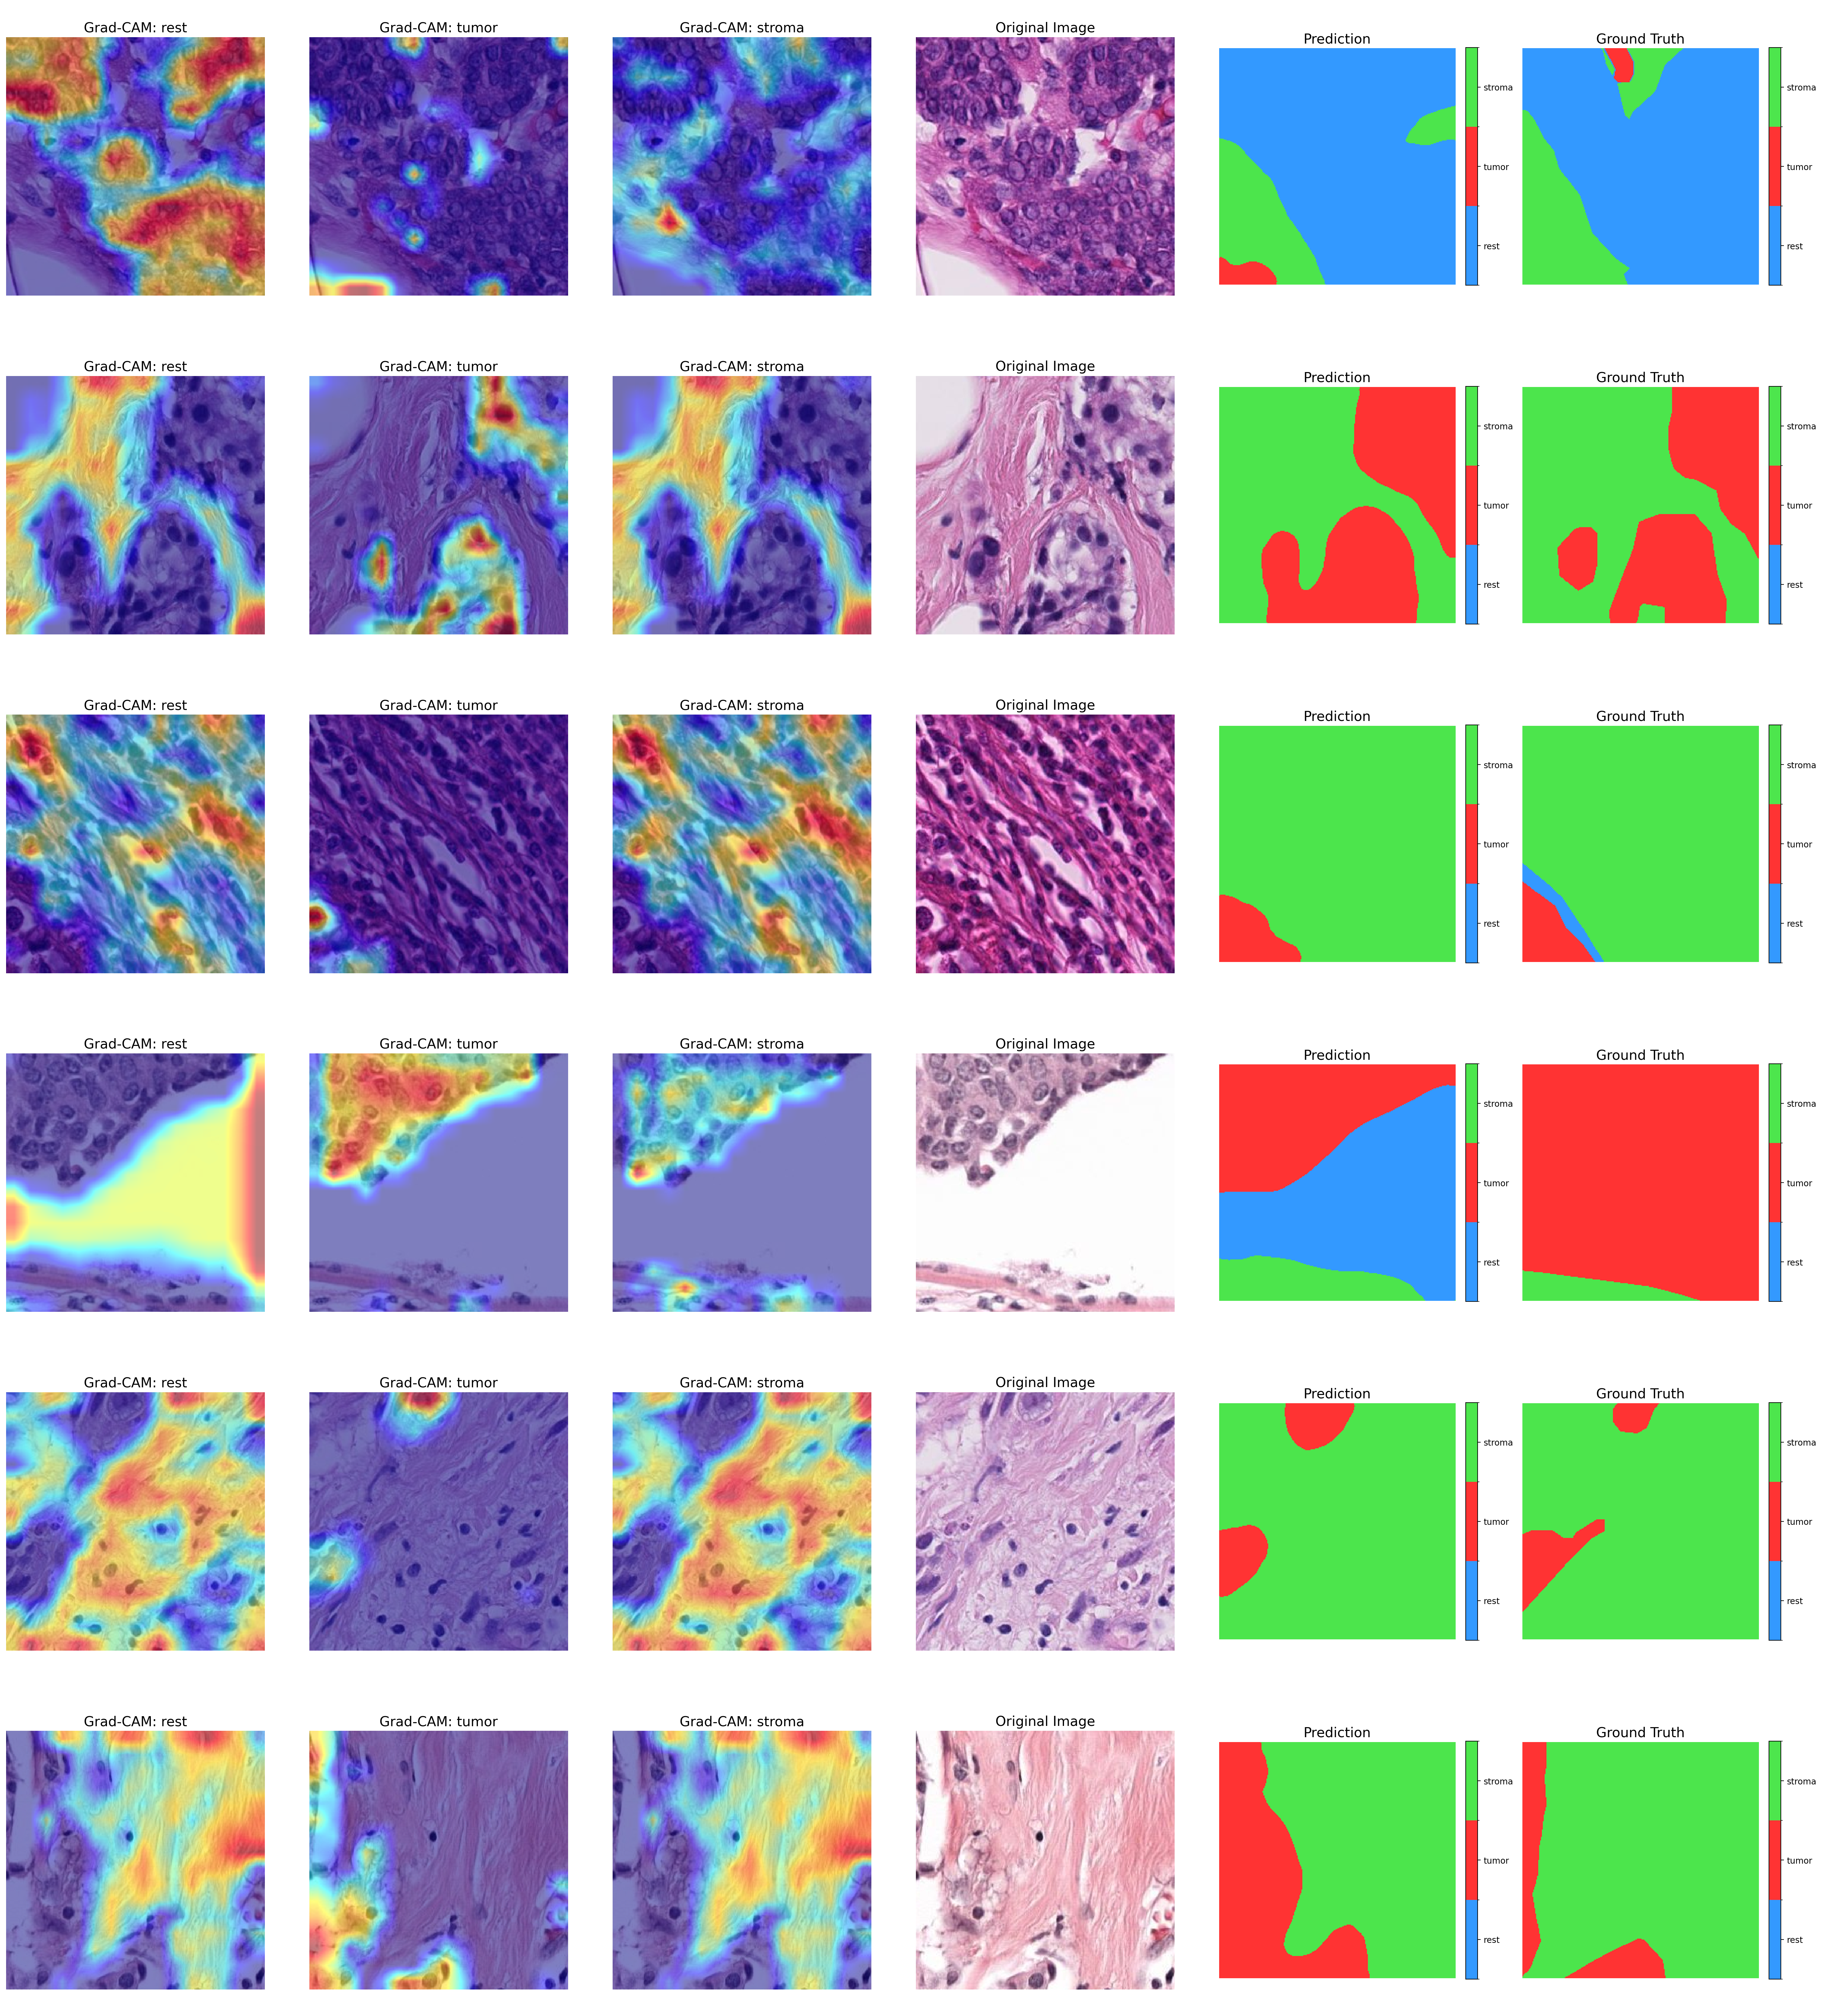
\includegraphics[width=1.0\textwidth]{images/gradcam-2.png}%
    }
    \caption{ GradCAM of Attention U-Net}
    \label{fig:figure2}
\end{figure}

\end{document}